\documentclass[a4paper, 12pt]{article}
\usepackage[left=2cm, right=2cm, top=2cm, bottom=2cm]{geometry}
\setlength{\parindent}{0cm}
\usepackage{graphicx}
\begin{document}
\title{\vspace{3cm}MM2090: Introduction to Scientific Computing\\
\vspace{1cm}
Assignment 4}
\author{\vspace{1cm}
\\Nayanatara MM20B042}
\date{\vspace{1cm}\today}
\maketitle
\newpage
\tableofcontents
\listoffigures

\vspace{5cm}
\section{Nayanatara (MM20B042)}

\vspace{0.5cm}
\subsection{What is the Coulomb's Law?}
Electrostatic force is one of the fundamental forces of nature. Coulomb's law states that electrostatic force of attraction or repulsion between two static point charges is directly proportional to the product of the magnitude of charges and inversely proportional to the square of the distance between them.
\\The mathematical equation of Coulomb's law is:

\begin{equation}
	F = \frac{kq_1q_2}{r^2}
	\label{eqn:1}
\end{equation}
Here, 'k' is known as Coulomb's constant. 

\begin{figure}[h]
	\begin{center}
		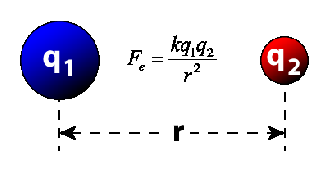
\includegraphics[scale=1.5]{mm20b042.eps}
	\end{center}
	\caption{Coulomb's Law}
	\label{fig1}
\end{figure}

'$q_1$' and '$q_2$' are the values of charges on the two charged particles and 'r' is the distance between them as shown in the figure \ref{fig1}.

\subsection{Different terms used in Coulomb's Law}
\begin{itemize}

	\item $k$ is a proportionality constant that appears in the equation. Known as Coulomb's constant, it's value in SI units is approximately equal to $9*10^9 N m^{2} kg^{-2}$.
	\item '$q_1$' and '$q_2$' are the values of charges on two charged particles between which the electrostatic force is being calculated. SI unit is Coulombs.
	\item '$r$' is the perpendicular distance between the two charged particles. SI unit is metres. 
	\item '$F$' in equation \ref{eqn:1} is the Electrostatic Force. SI unit for force is Newton. The electrostatic force acts only between charged particles. The force can be attractive or repulsive depending on the nature of the charges. Like charges repel each other while opposite charges attract. From equation \ref{eqn:1}, if 'F' has a negative value, then the force is attractive in nature and if it is positive then the force is repulsive in nature. "This introduces a difference in sign in corresponding equations such as those for field intensity, potential and the statement of Gauss's law. It also causes a differential action of the electric field on the positive and negative charges that constitute matter, giving rise to electric polarization, which has no gravitational analog"~\cite{Murdock1944}.
	
\end{itemize}

\subsection{Importance of Coulomb's Law}

Coulomb's law is significant in understanding everything from static electricity to the interactions between atomic nuclei.
Two nuclei would repel each other unless they are close enough for nuclear forces to attract. This explains why high energies are required to fuse nuclei. Electrostatic force is the reason why atoms are stable in the first place.


\bibliography{MM20B042}
\bibliographystyle{plain}



\end{document}
